%%%%%%%%%%%%%%%%%%%%%%%%%%%%%%%%%%%%%%%%%
% Short Sectioned Assignment
% LaTeX Template
% Version 1.0 (5/5/12)
%
% This template has been downloaded from:
% http://www.LaTeXTemplates.com
%
% Original author:
% Frits Wenneker (http://www.howtotex.com)
%
% License:
% CC BY-NC-SA 3.0 (http://creativecommons.org/licenses/by-nc-sa/3.0/)
%
%%%%%%%%%%%%%%%%%%%%%%%%%%%%%%%%%%%%%%%%%

%----------------------------------------------------------------------------------------
%	PACKAGES AND OTHER DOCUMENT CONFIGURATIONS
%----------------------------------------------------------------------------------------

\documentclass[paper=a4, fontsize=11pt]{scrartcl} % A4 paper and 11pt font size

\usepackage[T1]{fontenc} % Use 8-bit encoding that has 256 glyphs
%\usepackage{fourier} % Use the Adobe Utopia font for the document - comment this line to return to the LaTeX default
\usepackage[english]{babel} % English language/hyphenation
\usepackage{amsmath,amsfonts,amsthm} % Math packages
\usepackage{mathtools} %More math! (For dscases)
\usepackage{hyperref} %HTML package
\usepackage{pgfplots} %Makes plots in LaTeX
\usepackage{tikz} %Also tikz?
\usepackage{bbm} %Blackboard bold 1
\usepgfplotslibrary{fillbetween}%Let's me fill between named plots
\usepackage{graphicx} %import pics
\usepackage{bm} %vectors
\graphicspath{ {Python_figs/} }
\DeclareGraphicsExtensions{.pdf,.png,.jpg}
\usepackage{sectsty} % Allows customizing section commands
\allsectionsfont{ \normalfont\scshape} % Make all sections the default font and small caps


\renewcommand{\thesubsection}{\alph{subsection}} %Make subsections start with letters

\usepackage{fancyhdr} % Custom headers and footers
\pagestyle{fancyplain} % Makes all pages in the document conform to the custom headers and footers
\fancyhead{} % No page header - if you want one, create it in the same way as the footers below
\fancyfoot[L]{} % Empty left footer
\fancyfoot[C]{} % Empty center footer
\fancyfoot[R]{\thepage} % Page numbering for right footer
\renewcommand{\headrulewidth}{0pt} % Remove header underlines
\renewcommand{\footrulewidth}{0pt} % Remove footer underlines
\setlength{\headheight}{13.6pt} % Customize the height of the header

\numberwithin{equation}{section} % Number equations within sections (i.e. 1.1, 1.2, 2.1, 2.2 instead of 1, 2, 3, 4)
\numberwithin{figure}{section} % Number figures within sections (i.e. 1.1, 1.2, 2.1, 2.2 instead of 1, 2, 3, 4)
\numberwithin{table}{section} % Number tables within sections (i.e. 1.1, 1.2, 2.1, 2.2 instead of 1, 2, 3, 4)

\setlength\parindent{0pt} % Removes all indentation from paragraphs - comment this line for an assignment with lots of text

\usepackage{listings}
\lstset{language=Python}
%----------------------------------------------------------------------------------------
%	TITLE SECTION
%----------------------------------------------------------------------------------------

\newcommand{\horrule}[1]{\rule{\linewidth}{#1}} % Create horizontal rule command with 1 argument of height

\title{	Assignment 10}

\author{Benjamin Jakubowski} % Your name

\date{\normalsize\today} % Today's date or a custom date

\begin{document}

\maketitle % Print the title

%----------------------------------------------------------------------------------------
%	PROBLEM 1
%----------------------------------------------------------------------------------------

\section{Statements}

\subsection{Subspaces}
Statement 1: For any subspace $\mathcal{S}$ belonging to a vector space $\mathcal{V}$ of dimension $n$
\[ \mathrm{dim} (\mathcal{S}) + \mathrm{dim} (\mathcal{S^{\perp}}) = n\]

Proof:\\
Let $\{s_1, s_2, ..., s_j\}$ be an orthonormal basis for the subspace $\mathcal{S}$. Note that $\mathrm{dim}(\mathcal{S}) = j$. Now let $\{v_1, v_2, ..., v_n\}$ be a basis for the vector space $\mathcal{V}$. Then, using Gram-Schmidt, we can construct an orthonormal basis for $\mathcal{V}$ that includes the basis vectors for $\mathcal{S}$:
\[\{s_1, s_2, ..., s_j, w_1, w_2, ..., w_{n-j}\}\]
where the $w_i$'s are unit norm, linearly independent vectors constructed as linear combinations of the original basis vectors vectors $v_1, v_2, ..., v_n$. \\

Now take $y \in \mathcal{S}^{\perp}$. Then, since $y \in \mathcal{V}$, we know:
\[ y = \sum_{i = 1}^{j} \alpha_i s_i + \sum_{k=1}^{n - j} \beta_k w_k\]

Since $y \in \mathcal{S}^{\perp}$, we know that $\alpha_i = 0$ for all $i \in \{1, ..., j\}$. Thus y is a linear combination of the $w_k$'s. But then, since $y$ was arbitrary, we know that $\mathcal{S}^{\perp}$ is spanned by $\{w_1, w_2, ..., w_{n-j}\}$. Finally, by construction we know the $w_i$'s are linearly independent, so $\{w_1, w_2, ..., w_{n-j}\}$ is a basis for $\mathcal{S}^{\perp}$. Thus, $\textrm{dim}(\mathcal{S}^{\perp}) = n-j$ and

\[ \mathrm{dim} (\mathcal{S}) + \mathrm{dim} (\mathcal{S^{\perp}}) = n\] \qed

\subsection{Dimensions of the null space and range of $A$}

Statement 2:
\[\mathrm{dim}(\mathrm{null}(A)) + \mathrm{dim}(\mathrm{range}(A)) = n\]

Proof:\\

By Lemma 1.5 (in lecture notes 10),
\[\mathrm{null}(A) = \mathrm{row}(A)^{\perp}\]
Then, by statement (a) (proved above),
\[\mathrm{dim}(\mathrm{row}(A)^{\perp})+ \mathrm{dim}(\mathrm{row}(A)) = n\]

But (by Theorem 6.2 in lecture notes 9), $\mathrm{dim}(\mathrm{row}(A)) = \mathrm{dim}(\mathrm{col}(A))$. Thus,
\begin{align*}
\mathrm{dim}(\mathrm{row}(A)^{\perp})+ \mathrm{dim}(\mathrm{row}(A)) &= n \\
 \implies \qquad{} \mathrm{dim}(\mathrm{row}(A)^{\perp}) + \mathrm{dim}(\mathrm{col}(A)) &= n \\
\implies \qquad{}\mathrm{dim}(\mathrm{null}(A)) + \mathrm{dim}(\mathrm{col}(A)) &=n \qed
\end{align*}

\subsection{$A^T(AA^T)^{-1}Ax$ as projection onto row space of full-rank, fat A}

Statement: For any full-rank matrix $A \in \mathbb{R}^{m \times n}, m \leq n, A^T(AA^T)^{-1}Ax$ is the projection of $x \in \mathbb{R}^n$ onto the row space of $A$. \\

Proof: \\

First, note $A^T$ is a full-rank matrix in $\mathbb{R}^{n \times m}, n \geq m$. Therefore, by Theorem 2.2 in Lecture notes 10, we know:

\[\mathcal{P}_{\textrm{range}(A^T)} x = (A^T)((A^T)^T(A^T))^{-1}(A^T)^Tx = A^T(AA^T)^{-1}Ax\]

Then merely noting $\textrm{range}(A^T) = \textrm{row}(A)$ yields the desired result:
\[\mathcal{P}_{\textrm{row}(A)} x =  A^T(AA^T)^{-1}Ax\] \qed

As a side note, we can perhaps better understand this projection by decomposing the expression into two pieces:
\begin{align*}
\mathcal{P}_{\textrm{row}(A)} x &=  A^T(AA^T)^{-1}Ax \\
   &= \left[\begin{matrix} A_{\textrm{row 1}} \ A_{\textrm{row 2}} \ \dots \ A_{\textrm{row m}} \end{matrix}\right] \underbrace{(AA^T)^{-1}Ax}_{\text{Coordinates of $x$ w.r.t. row's of $A$}}
\end{align*}

\subsection{Regression with an orthogonal matrix }

Statement 4: If the columns of $A \in \mathbb{R}^{m \times n}, m \geq n$, are orthonormal then the solution to the least-squares problem is of the form
\[x = \mathrm{arg} \min_z ||y - Az||_2 = A^T y\]

Proof: \\

If the columns of $A \in \mathbb{R}^{m \times n}, m \geq n$ are orthonormal, than $A$ is an orthogonal matrix. But then,
\[ A A^T = \mathbf{1}_n\]
so
\[A (A^Ty) = (AA^T)y = \mathbf{1}_n y = y\]
So the least squares solution to the equation $Ax = y$ is
\[x_{LS} = \arg \min_z ||y - Az||_2 = A^Ty\] \qed

%----------------------------------------------------------------------------------------
%	PROBLEM 2
%----------------------------------------------------------------------------------------

\section{Global Warming}

\subsection{Completed hw10\_pb2.py script}

Here are the scripts necessary to  fit the models:\\

\begin{lstlisting}[frame=single, basicstyle=\small]

# First build matrix A:
import pandas as pd


t = np.arange(n)
A = pd.concat([pd.Series(np.ones(n).T, name='One'),\
               pd.Series(np.cos(2.0*np.pi*t/12.0).T, name='Cos'),\
               pd.Series(np.sin(2.0*np.pi*t/12.0).T, name='Sin'),\
               pd.Series(t.T, name='Month')], axis=1)
               
#Then fit models
max_model_coef = np.linalg.lstsq(A.values, max_temp)[0]
def max_model(t):
    y_fit = max_model_coef[0] +\
    max_model_coef[1]*np.cos(2.0*np.pi*t/12.0) +\
    max_model_coef[2]*np.sin(2.0*np.pi*t/12.0) +\
    max_model_coef[3]*t
    return y_fit

def max_trend(t):
    y_fit = max_model_coef[0] + max_model_coef[3]*t
    return y_fit

min_model_coef = np.linalg.lstsq(A.values, min_temp)[0]
def min_model(t):
    y_fit = min_model_coef[0] +\
    min_model_coef[1]*np.cos(2.0*np.pi*t/12.0) +\
    min_model_coef[2]*np.sin(2.0*np.pi*t/12.0) +\
    min_model_coef[3]*t
    return y_fit

def min_trend(t):
    y_fit = min_model_coef[0] + min_model_coef[3]*t
    return y_fit

reconstruction_max = max_model(t)
reconstruction_min = min_model(t)
trend_max =  max_trend(t)
trend_min =  min_trend(t)
\end{lstlisting}

\subsection{Hypothesis Test}

Recall we fit the same model to data from 100 stations and observe the slope is positive for 65 stations. We are interested in testing:
\begin{align*}
\mathcal{H}_0: & \qquad{}  \beta_{linear} = 0 \\
\mathcal{H}_A: & \qquad{} \beta_{linear} \ne 0
\end{align*}
Under our null hypothesis, the number of observations with $\beta_{linear} > 0$ is distributed as a binomial random variable $X$ with $n = 100$ and $p = 0.5$. Thus, conservatively using a two-sided hypothesis test, we get
\begin{align*}
P &= P(X \leq 35 \textrm{ or } X\geq 65) \\
   &= P(X \leq 35) + P(X \geq 65) \\ 
   &= \sum_{i = 0}^{35}{100 \choose i} \cdot 0.5^{100} + \sum_{i = 65}^{100}{100 \choose 35} \cdot 0.5^{100} \\
   &= 0.00176 + 0.00176 = 0.00352
\end{align*} 

Thus we have strong evidence of warming if 65 of 100 stations record data yield positive $\beta_{linear}$.

%----------------------------------------------------------------------------------------
%	PROBLEM 3
%----------------------------------------------------------------------------------------

\section{Weight prediction}

\subsection{Least-squares estimate of $\alpha$ without intercept}

Using theorem 2.2, the least squares estimate of $\alpha$ is:

\begin{align*}
\alpha_{LS} &= (w^T \cdot w)^{-1}\cdot w^T \cdot h \\
\end{align*}

\subsection{Adding an intercept}

The point of adding an intercept is to give the linear model an additional degree of freedom. Without the intercept term (in a 2D data set), the regression line is constrained to pass through the origin. Adding an intercept terms removes this constraint, allowing the regression model to capture any linear relationship in $\mathbb{R}^2$. This is illustrated below using simulated data:

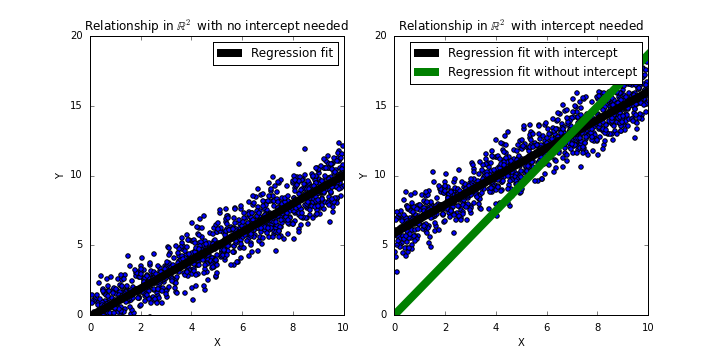
\includegraphics[scale = 0.6]{Q3B_fig.png}

\subsection{Models with and without intercept for heigh/weight}

After completing the script $hw10\_pb2.py$, the relative errors achieved by the two models on the test dataset are:

\begin{enumerate}
\item Model 1 (no intercept) relative error: 0.06295
\item Model 2 (with intercept) relative error: 0.01951
\end{enumerate}

The model with the intercept terms has much lower relative error, so adding the intercept clearly improves the model.

\subsection{Models with and without intercept for height/weight}

To compare the performance of the two models on the height weight test set, the following simulations were conducted:
\begin{itemize}
\item For $n \in \{2, 100\}, n$ observations were randomly sampled from the data to form the test set.
\item Both models were fit, and the relative error was determined using  $21000 - n$ held-out observations.
\item This was repeated 10 times, and the mean and standard deviation of the relative error was calculated for each $n$.
\end{itemize}

Results from these simulations are shown below:

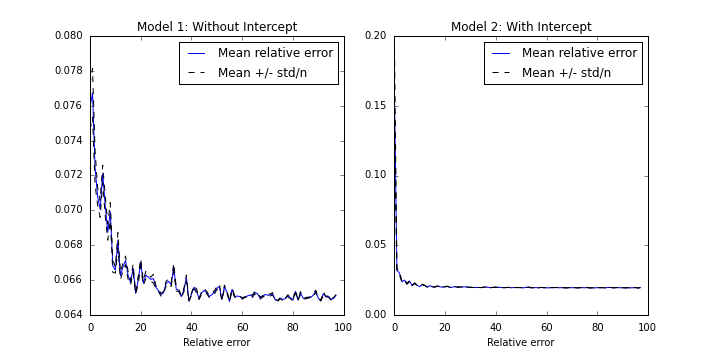
\includegraphics[scale = 0.6]{Q3D_fig.png} 

As you can see, including the intercept results in improved model performance on all but the very smallest $n$. In fact, the no-intercept model only outperformed the intercept model when $n = 2$. Given this $n$ is absurd (in no realistic situation would you try fitting a model to two observations), these results suggest including an intercept produces better results when less data is available. \\

In general, I would favor linear models when less data is available. This is because allowing non-linearity may lead to overfitting, and this is more likely when less data is available. When more data is available, we are better able to control overfitting (through use of hold-out validation sets, for example) and can introduce more complexity into our model. When less data is available, the constraint imposed by the linearity requirement helps avoid overfitting.


%----------------------------------------------------------------------------------------
%	PROBLEM 4
%----------------------------------------------------------------------------------------

\section{Noise Amplification}

\emph{Note: This problem was completed with significant assistance from Professor Fernandez-Granda, Nora, Mike, Filipe, and the other students present at the Professor's office hours on 12/2/15.}

\subsection{Least-squares solution}

Recall we are interested in estimating a vector $x \in \mathbb{R}^n$ from data $y \in \mathbb{R}^m, m \geq n$, that we know follows the model
\[y = Ax + z\]
where $A \in \mathbb{R}^{m \times n}$ is full rank.

We aim to find the least-squares solution $x_{LS}$ in terms of the SVD of $A, z$, and $x$.

First, we know:
\[x_{LS} = VS^{-1}U^T y\]
where $USV^T$ is the SVD of $A$.
Then, substituting for $y$ yields
\[x_{LS} = VS^{-1}U^T (Ax + z) = VS^{-1}U^T (USV^Tx + z) = x + VS^{-1}U^Tz \]

\subsection{Maximizing the estimation error}

Now we are interested in finding $z$ with unit $\ell_2$ norm that maximizes the estimation error $||x_{LS} - x||_2$. Note this is equavelent to maximizing $||x_{LS} - x||_2^2$.

First, substituting in the expression from (a) yields:
\[||x_{LS} - x||_2^2 = || (x + VS^{-1}U^Tz) - x||_2^2 = ||VS^{-1}U^Tz ||_2^2 \]

Now, since $V$ is an orthogonal matrix, we know
\[||VS^{-1}U^Tz ||_2^2 = ||S^{-1}U^Tz ||_2^2\]

Next, before we proceed, let's introduce some notation- let $u_i$ represent the $i^{\text{th}}$ column of $U$, such that $U = \left[ \begin{matrix} u_1 \ u_2 \ \dots \ u_n \end{matrix} \right]$. Then expanding yields
\begin{align*}
||S^{-1}U^Tz ||_2^2 &=
\left|\left|
\left[\begin{matrix}
\frac{1}{\sigma_1} \ \qquad{} \ \qquad{}  \\
\qquad{} \ \ddots \ \qquad{} \\
\qquad{}  \ \qquad{}  \ \frac{1}{\sigma_n}
 \end{matrix}\right]
  \left[\begin{matrix}
u_1^T z  \\
\vdots \\
u_n^T z
\end{matrix}\right]
 \right|\right|_2^2 \\
 &=\left|\left|
 \left[\begin{matrix}
\frac{u_1^T z}{\sigma_1}  \\
\vdots \\
\frac{u_n^T z}{\sigma_n}
\end{matrix}\right]
 \right|\right|_2^2 \\
 &= \sum_{i=1}^n \left(\frac{u_n^T z}{\sigma_i}\right)^2 \\ 
\end{align*}
Now (noting the columns of $U$ form an orthonormal basis for $\mathbb{R}^n$), let
\[z = \sum_{i = 1}^{n}\alpha_i u_i\]
Then note, for all $1 \leq k \leq n$, 
\[u_k^T z = u_k^T \sum_{i = 1}^{n}\alpha_i u_i = \sum_{i = 1}^{n}\alpha_i u_k^T u_i = \alpha_k\]
so
\begin{align*}
 ||S^{-1}U^Tz ||_2^2 &= \sum_{i=1}^n \left(\frac{u_n^T z}{\sigma_n}\right)^2 \\ 
    &= \sum_{i=1}^n \left(\frac{\alpha_i}{\sigma_i}\right)^2
\end{align*}
Then, note that for all $1 \leq i \leq n, \left(\frac{\alpha_i}{\sigma_i}\right)^2 \leq \left(\frac{\alpha_i}{\sigma_{min}}\right)^2$. Thus, 
\begin{align*}
\sum_{i=1}^n \left(\frac{\alpha_i}{\sigma_i}\right)^2 &\leq \sum_{i=1}^n \left(\frac{\alpha_i}{\sigma_{min}}\right)^2 \\
   &= \left(\sum_{i=1}^n \alpha_i^2\right) / \sigma_{min}^2
\end{align*}

But, since the $z$ has unit norm, we know $\sum_{i=1}^n \alpha_i^2 = 1$. Thus, we have
\[||x_{LS} - x||_2^2 = ||S^{-1}U^Tz ||_2^2 \leq \frac{1}{\sigma_{min}^2}\]

Thus, to maximize the error, we want $z$ to be in the direction of $u_{min}$, the left singular vector corresponding to the least singular value- in other words, we want
\[z = \sum_{i = 1}^{n}\alpha_i u_i = 1\cdot u_{min} + \sum_{\begin{matrix} i=1 \\ i \ne \text{min} \end{matrix}}^n 0 \cdot u_i\]

In the case of our example matrix
\[ A =
\left[
\begin{matrix}
2.1 \ 1.1 \\
3.2 \ 1.6 \\
2.4 \ 1.2 \\
\end{matrix}
\right]
\]
the corresponding left singular vector (found using WolframAlpha) is 
\[ u_{\text{min}} =
\left[
\begin{matrix}
0.883558 \\
-0.374658 \\
-0.280993 \\
\end{matrix}
\right]
\]
This vector corresponds to the minimum singular value of $\sigma_{min} = 0.0395142$. Hence, the maximum error is
\[{||x_{LS} - x||_2}_{\text{max}} = \frac{1}{0.0395142} = 25.3\]

\subsection{Ridge regression}

In ridge regression, we optimize the cost function
\[\min_x ||Ax - y||_2^2 + \gamma^2 ||x||_2^2\]

Our goal is to rewrite this as a least-squares problem of the form
\[\min_x ||Bx - c||_2\]
First, note for arbitrary matrices $G, H$ $||G||_2^2 + ||H||_2^2 = \left|\left| \left[ \begin{matrix}G\\H\end{matrix} \right] \right|\right|_2^2$. Thus,
\begin{align*}
||Ax - y||_2^2 + \gamma^2 ||x||_2^2 &= ||Ax - y||_2^2 +||\gamma x||_2^2 \\
   &= ||Ax - y||_2^2 +||\gamma \mathbb{I}_n x||_2^2 \\
   &= \left|\left| \left[ \begin{matrix}Ax - y\\ \gamma \mathbb{I}_n x \end{matrix} \right] \right|\right|_2^2 \\
   &= \left|\left| \left[ \begin{matrix}A\\ \gamma \mathbb{I}_n \end{matrix} \right] x - \left[ \begin{matrix}y\\ \bm{0} \end{matrix} \right] \right|\right|_2^2
\end{align*}
where $\bm{0}$ is $n \times 1$. Moreover, note that
\begin{itemize}
\item $ \left[ \begin{matrix}A\\ \gamma \mathbb{I}_n \end{matrix} \right] $ is $(m+n) \times n$
\item $\left[ \begin{matrix}y\\ \bm{0} \end{matrix} \right]$ is $(m+n)$.
\end{itemize}

\subsection{Expression for $x_{RR}$}

We aim to show that
\[x_{RR} := \sum_{i=1}^n \frac{\sigma_i}{\sigma_i^2 + \gamma^2}(\sigma_i v_i^T x + u_i^T z)v_i\]

We proceed by expanding the least-squares form of ridge regression:
\begin{align*}
x_{RR} &= \min_x ||Ax - y||_2^2 + \gamma^2 ||x||_2^2 \\
   &=\min_x \left|\left| \left[ \begin{matrix}A\\ \gamma \mathbb{I}_n \end{matrix} \right] x - \left[ \begin{matrix}y\\ \bm{0} \end{matrix} \right] \right|\right|_2^2 \\
   &= \left( \left[ \begin{matrix}A\\ \gamma \mathbb{I}_n \end{matrix} \right]^T  \left[ \begin{matrix}A\\ \gamma \mathbb{I}_n \end{matrix} \right] \right)^{-1}  \left[ \begin{matrix}A\\ \gamma \mathbb{I}_n \end{matrix} \right] ^T \left[ \begin{matrix}y\\ \bm{0} \end{matrix} \right]\\
   &= \left( \left[A^TA + \gamma^2\mathbb{I}_n\right]\right)^{-1} \left[A^Ty\right] \\
   &= \left(\left[(VSU^T)(USV^T) + \gamma^2 \mathbb{I}_n\right]\right)^{-1}\left[A^Ty\right]  \\
   &= \left(\left[VS^2V^T + \gamma^2 \mathbb{I}_n\right]\right)^{-1}\left[A^Ty\right] \\
   &= \left(\left[VS^2V^T + \gamma^2 VV^T\right]\right)^{-1}\left[A^Ty\right] \\
   &= \left( V \left[S^2 + \gamma^2 \mathbb{I}_n\right] V^T\right)^{-1} \left[A^Ty\right] \\
   &= V^{-T} \left[S^2 + \gamma^2 \mathbb{I}_n\right]^{-1} V^{-1} \left[A^Ty\right] \\
   &= V \left[S^2 + \gamma^2 \mathbb{I}_n\right]^{-1} V^{T} \left[A^Ty\right] \\
   &= V \left[S^2 + \gamma^2 \mathbb{I}_n\right]^{-1} V^{T} \left[(VSU^T)y\right] \\
   &= V \left[S^2 + \gamma^2 \mathbb{I}_n\right]^{-1} SU^Ty \\
   &= V \left[S^2 + \gamma^2 \mathbb{I}_n\right]^{-1} SU^T(Ax+z) \\
   &= V \left[S^2 + \gamma^2 \mathbb{I}_n\right]^{-1} SU^T(USV^Tx+z) \\
   &= V \left[\begin{matrix}
\frac{\sigma_1}{\sigma_1^2 + \gamma^2} \ \qquad{} \  \bm{0}  \\
\qquad{} \ \ddots \ \qquad{} \\
 \bm{0}  \ \qquad{}  \ \frac{\sigma_n}{\sigma_n^2 + \gamma^2}
 \end{matrix}\right]U^T(USV^Tx+z)\\
    &= V \left[\begin{matrix}
\frac{\sigma_1}{\sigma_1^2 + \gamma^2} \ \qquad{} \  \bm{0}  \\
\qquad{} \ \ddots \ \qquad{} \\
 \bm{0}  \ \qquad{}  \ \frac{\sigma_n}{\sigma_n^2 + \gamma^2}
 \end{matrix}\right](SV^Tx+U^Tz) \\
        &=  \sum_{i=1}^n \frac{\sigma_i}{\sigma_i^2 + \gamma^2}(\sigma_i v_i^T x + u_i^T z)v_i
\end{align*}

\subsection{Separating the error term into two components}

Our goal is to separate the error term $||x - x_{RR}||_2$ into two components- one that increases and one that decreases with $\gamma$.

\begin{align*}
x - x_{RR} &= x - \sum_{i=1}^n \frac{\sigma_i}{\sigma_i^2 + \gamma^2}(\sigma_i v_i^T x + u_i^T z)v_i \\
   &= \left[ x - \sum_{i=1}^n \frac{\sigma_i}{\sigma_i^2 + \gamma^2}(\sigma_i v_i^T x v_i )\right]+ \left[\sum_{i=1}^n \frac{\sigma_i}{\sigma_i^2 + \gamma^2}(u_i^T z)v_i \right]
\end{align*}

Now, note that the $v_i$'s form an orthonormal basis- thus, we can express
\[x = \sum_{i=1}^n v_i^T x v_i\]
Substituting yields
\begin{align*}
x - x_{RR} &= \left[ \sum_{i=1}^n v_i^T x v_i - \sum_{i=1}^n \frac{\sigma_i}{\sigma_i^2 + \gamma^2}(\sigma_i v_i^T x v_i )\right]+ \left[\sum_{i=1}^n \frac{\sigma_i}{\sigma_i^2 + \gamma^2}(u_i^T z)v_i \right] \\
   &=\left[ \sum_{i=1}^n \left(1 - \frac{\sigma_i^2}{\sigma_i^2 + \gamma^2}\right) (v_i^T x v_i )\right]+ \left[\sum_{i=1}^n \frac{\sigma_i}{\sigma_i^2 + \gamma^2}(u_i^T z)v_i \right] \\
   &=\underbrace{\left[ \sum_{i=1}^n \left( \frac{\gamma^2}{\sigma_i^2 + \gamma^2}\right) (v_i^T x v_i )\right]}_{\text{Component 1: Increases with $\gamma$}}+ \underbrace{\left[\sum_{i=1}^n \frac{\sigma_i}{\sigma_i^2 + \gamma^2}(u_i^T z)v_i \right]}_{\text{Component 2: Decreases with $\gamma$}}
\end{align*}

\subsection{Value of ridge regression when matrix $A$ is badly conditioned}

As shown above, there are two components of the error. If the matrix is badly conditioned, then (holding $\gamma$ constant) component 2 is expected to be large. In response, we can increase $\gamma$ to reduce the contribution of component 2 to error. This biases our estimate, but reduces our overall error (up until the point when the error reduction achieved by decreasing component 2 is less than the error augmentation caused by increasing component 1). Because there is this trade off, we should optimize $\gamma$ through cross-validation (for example).
%----------------------------------------------------------------------------------------
\end{document}